\documentclass[11pt]{article}
\usepackage[table]{xcolor}  % load xcolor before anything else
\usepackage[most]{tcolorbox}
\usepackage{setspace}  %line spacing
\usepackage{titling}
\usepackage{graphicx}
\usepackage{parskip}    %spaced paragraphs
\usepackage{csquotes}   %babel wanted it
% \usepackage{emptypage} % prevent page numbers and headings on empty pages
\usepackage{float} % for H specification
% \usepackage{censor}
\usepackage{amsmath}
% \usepackage{fontawesome}
% \usepackage{pdfpages} % insert pdf 
% \usepackage[titletoc]{appendix}
\usepackage{pdflscape} % landscape pdf pages
\usepackage{wrapfig}
\usepackage{booktabs,nicematrix} % quality tables 

\usepackage{circuitikz}
\usetikzlibrary{calc}

\usepackage[hang,flushmargin]{footmisc}     % footnote editing

\usepackage[font=small,labelfont=bf,justification=centering]{caption} % caption size 
\usepackage{subcaption}
\setlength{\belowcaptionskip}{-5pt}

\usepackage[hidelinks]{hyperref}  %have a review of this
\hypersetup{%
%   citecolor=black,
  colorlinks=false,
%   linkcolor=black,
%   urlcolor=black
}
\usepackage[nameinlink]{cleveref}

\usepackage{listings}% code
\definecolor{codegreen}{rgb}{0,0.6,0}
\definecolor{codegrey}{rgb}{0.5,0.5,0.5}
\definecolor{codepurple}{rgb}{0.58,0,0.82}
\definecolor{backcolour}{rgb}{0.95,0.95,0.92}
\lstdefinestyle{codestyle}{
    backgroundcolor=\color{backcolour},   
    commentstyle=\color{codegrey},
    keywordstyle=\color{blue},
    numberstyle=\tiny\color{codegrey},
    stringstyle=\color{codegreen},
    basicstyle=\ttfamily\lst@ifdisplaystyle\footnotesize\fi,
    breakatwhitespace=false,         
    breaklines=true,                 
    captionpos=t,                    
    keepspaces=true,                 
    % numbers=left,                    
    numbersep=5pt,                  
    showspaces=false,                
    showstringspaces=false,
    showtabs=false,                  
    tabsize=2,
    framextopmargin=50pt,
    frame=bottomline,
    % belowcaptionskip=0pt,
    aboveskip=-1pt,
    belowskip=1pt
}
\lstset{style=codestyle}

\usepackage{geometry}
\geometry{a4paper, margin=1.5cm}

\usepackage{fontspec}
\setmainfont[ 
    Mapping=tex-text,
    BoldFont={HelveticaNowText-Bold},
    ItalicFont={HelveticaNowText-RegIta},
    BoldItalicFont={HelveticaNowText-BoldItalic}
]{[HelveticaNowText-Regular]}
\usepackage{unicode-math}
\setmathfont[mathrm=sym]{Fira Math}

\usepackage{fancyhdr}   %footer
\fancypagestyle{myheadings}{%
    \fancyhf{}
    \renewcommand{\headrulewidth}{0.5pt}
    \renewcommand{\footrulewidth}{0pt}
    \addtolength{\headheight}{2pt}
    % \fancyhead[L]{\leftmark}
    \fancyhead[L]{ES3D8}
    \fancyhead[R]{1922268}
    \cfoot{\thepage}
}
\pagestyle{myheadings}

\usepackage{enumitem}   %reduce list spacing
\setlist{nosep} 

\usepackage[
    backend=biber,
    % style=numeric-comp,
    % style = vancouver,
    % style = science,
    style = ieee,
    % style=draft,
    % style = authoryear-icomp,
    maxnames=2, minnames=2,
    % doi=false,
    sorting=none
]{biblatex}   %bibliography
\usepackage{xurl} % break urls. load after biblatex
\addbibresource{sections/refs.bib}

\usepackage[
    separate-uncertainty=true,
    multi-part-units=single
    ]{siunitx}
\sisetup{
    detect-all,
    per-mode=symbol-or-fraction,
    % tight-spacing,
    quantity-product =,
    number-unit-product=\,,
    % space-before-unit=false
}
\DeclareSIUnit{\mAh}{mAh}

\usepackage{xltabular}
\usepackage{multirow}
\newcolumntype{Y}{>{\centering\arraybackslash}X}
\newcolumntype{Z}{>{\raggedright\arraybackslash}X}
\newcolumntype{P}[1]{>{\centering\arraybackslash}p{#1}}

\newenvironment{conditions}[1][where:]
  {#1 \begin{tabular}[t]{>{$}l<{$} @{} >{${}}c<{{}$} @{} l}}
  {\end{tabular}\\[\belowdisplayskip]}

\definecolor{titlepagecolour}{HTML}{003D99}
\definecolor{tableh1}{HTML}{dae3eb} %table grey
\definecolor{tableh2}{HTML}{b3ccf5} %table bluegrey
\definecolor{titleblue}{HTML}{1b1787} % blue
\definecolor{tableg}{HTML}{309c3d} % green
\definecolor{tablea}{HTML}{ed901f} % amber
\definecolor{tabler}{HTML}{f2422e} % red

\usepackage[british]{babel} 

% \usepackage{pgfgantt}
% \setganttlinklabel{s-s}{}
% \setganttlinklabel{f-s}{}
% \setganttlinklabel{f-f}{}

\usepackage{titlesec} 
\titlespacing\section{0pt}{12pt plus 4pt minus 2pt}{0pt plus 2pt minus 2pt}
\titlespacing\subsection{0pt}{12pt plus 4pt minus 2pt}{0pt plus 2pt minus 2pt}
\titlespacing\subsubsection{0pt}{12pt plus 4pt minus 2pt}{0pt plus 2pt minus 2pt}
\titlespacing\paragraph{0pt}{10pt plus 4pt minus 2pt}{10pt plus 2pt minus 2pt}

\begin{document}
% \onehalfspacing
% \setstretch{1.25} % one and quarter spacing

\section{Introduction to VGA}\label{sec:intro}
VGA (Video Graphics Array) is a visual graphics standard introduced in 1987.
It was developed to work with CRT (Cathode-Ray Tube) technology, which works 
by drawing each pixel in horizontal lines vertically down the display to 
create a \emph{frame}.

In order to produce the effect of a static image 
given only a single pixel controlled per instant, the entire frame 
would be redrawn (or `refreshed') quicker than the eye can perceive.
A refresh rate of \qty{60}{\Hz} would be typical.

Due to the physical deflection of an electron beam to produce pixels, 
extra time for the beam to adjust to a new line is included in the standard, called 
the \emph{blanking interval}. 
The start of a new line is controlled by the horizontal sync (hsync) signal, with a 
new frame in turn controlled by a vertical sync (vsync) signal. The blanking intervals before 
and after these signals are respectively called the \emph{front porch} and \emph{back porch}. 
In modern standards like HDMI, this extra time has been retained and instead carries extra 
data like accompanying audio. 


\subsection{Driving the display}\label{sec:drivingdisplay}

There are four requirements for driving a VGA display:
\begin{enumerate}
    \item Clock signal driving the display signal counters.
    \item Horizontal and vertical signals, defining pixels.
    \item Drawing graphical elements to the screen.
    \item Physical video output to a display.
\end{enumerate}

\subsubsection{Clock}
The required display frequency clock can be calculated by:
\begin{align*}
    f_{\text{clock}} & = L_h \times L_v \times f_{r}
\end{align*}

\begin{conditions}
    L_h & = & horizontal lines, 1903 \\
    L_v & = & vertical lines, 931 \\
    f_{r} & = & refresh frequency, \qty{60}{\Hz} \\
\end{conditions}

% where: 
% \begin{tabular}[H]{ l c l}
%     $\lambda$ & $=$ & wavelength \\
%     $v$ & $=$ & velocity, which in this case will be $c$, the speed of light \\
%     $f$ & $=$ & frequency \\
% \end{tabular}\\

The results in a required clock frequency of \qty{106.30158}{\MHz}. 
The easiest method of producing clock signals in Verilog is to divide down the main 
processor clock to the required subdivision. In the case of the 
Nexys A7, the onboard clock is \qty{100}{\MHz} and thus cannot be divided down to 
a value that is greater. However, by using the Clocking Wizard IP provided by Xilinx, 
this can be produced. The caveat is that it will not be necessarily exact. 
In this case, the actual output clock is \qty{106.296}{\MHz}, which is within \qty{0.005}{\percent}.

\subsubsection{Signals}
In this implementation, the horizontal and vertical signals are controlled by counters 
operating at the overall display frequency, determining which pixel is being drawn. 
The counter values then determine the widths of each signal parameter.
The parameters are outlined in \cref{table:vgaparams}, which informs the display dimensions
as shown in \cref{fig:vga}.
\begin{xltabular}{\linewidth}{Y|YYYY}
    & Sync signal & Back porch & Display & Front porch \\
    \hline
    Horizontal & 151 & 384 & 1824 & 1903 \\
    \hline
    Vertical & 2 & 30 & 930 & 931 \\
    \hline
    \caption{VGA signal parameters}\label{table:vgaparams}
\end{xltabular}
The visible portion produces a display resolution of 1440x900. 

\begin{figure}[htbp]
    \centering
    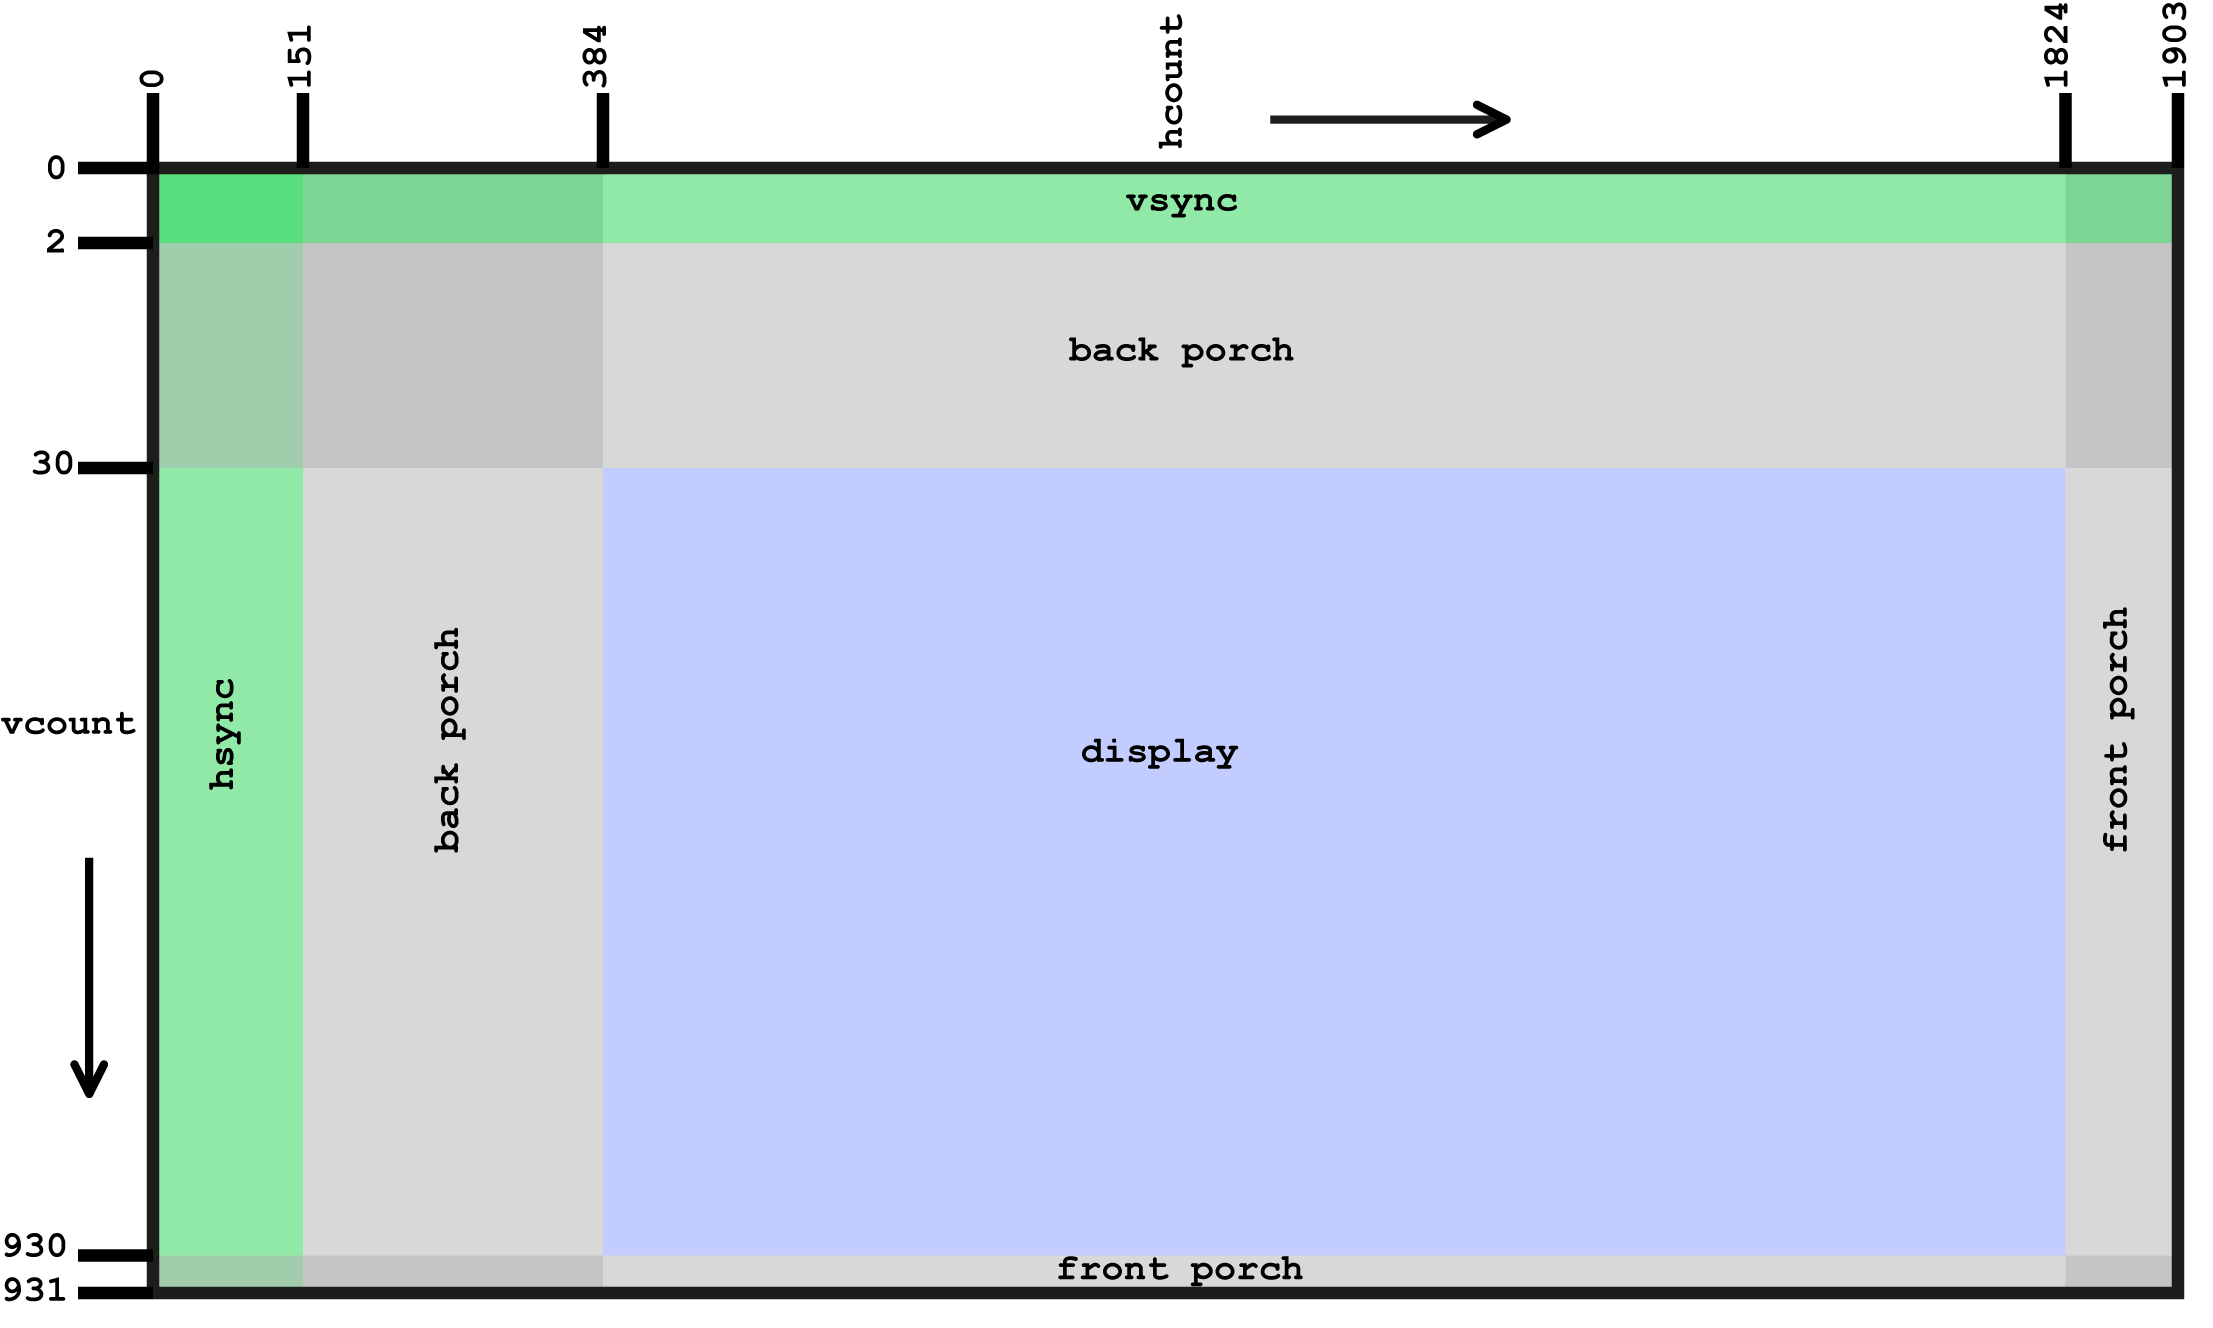
\includegraphics[width=0.8\textwidth]{./figures/vga display.png}
    \caption{Display parameters}\label{fig:vga}
\end{figure}

\subsubsection{Drawing graphics}
Graphics drawing is delegated to its own module\footnote{
    \Cref{sec:drawcon}.
} separate from the VGA controller. 
To provide an overview, the graphics drawing module (draw controller) takes as input the 
current pixel by coordinates in \emph{x} and \emph{y} with reference to the top left corner
of the visible display. It outputs the colour for this pixel as a 12-bit hexadecimal number, which can then 
be passed to the VGA port.

\subsubsection{Video output}
The specifics of the output (i.e. required voltages, pin connections etc. to the D-sub connector) is
abstracted away in the constraints file for the board. In this file, the pins of the Nexys A7 
with regard to the VGA port are provided and simply need to be 
included in the compilation to be used. 

The colour channels in the port are different physical connections, taking up six pins of the 
connector - one each for red, green, and blue, in addition to each colour's ground reference. 
In the implementation for this project, the 4-bit output colour variables
(\lstinline{VGA_R}, \lstinline{VGA_G}, \lstinline{VGA_B}) 
have been merged into a single 12-bit variable (\lstinline{colour}). 

The mapping occurs as follows:

\begin{tabular}{l|lll}
    Original & \lstinline|VGA_R[3:0]| & \lstinline|VGA_G[3:0]| & \lstinline|VGA_B[3:0]| \\
    Implementation & \lstinline|colour[11:8]| & \lstinline|colour[7:4]| & \lstinline|colour[3:0]| 
\end{tabular}
% \begin{lstlisting}[numbers=none,frame=none]
%         Original        |    VGA_R[3:0]     VGA_G[3:0]      VGA_B[3:0]
%         Implementation  |    colour[11:8]   colour[7:4]     colour[3:0] 
% \end{lstlisting}

The advantage of this is that colour assignment to a pixel can now be encoded as a single hexadecimal number 
with three digits - the first encoding the red value, the second green, and the third blue. 
This is particularly useful as the encoding now follows web-safe hexadecimal colour space\footnote{
    A palette reference available at \href{https://www.rapidtables.com/web/color/Web_Safe.html}{RapidTables \faExternalLink}.
}, reducing the guesswork in developing a colour on screen.

\subsection{Limitations}
With VGA as the only display adapter available on the board, the colours available is limited 
to 4-bits for the red, green, and blue channels each. This results in 4096 total colours. 
Most modern monitor displays, on the other hand, permit over 16 million colours due to the 
use of 24-bit colour space. 

\subsection{Implementation}
The implementation of the VGA controller can be found in \cref{code:vga}.

\clearpage
\section{Gate development}

In total five different gate cells are required. The process of designing a logic gate involves four major steps:
\begin{enumerate}
    \item Schematic design of transistor circuit.
    \item Simulation to verify the schematic is correct for the logic desired.
    \item Layout of silicon to produce the fabricable gate. 
    \item Simulation of the layout to verify it matches the schematic logic.
\end{enumerate}
The following section compares the schematic design to the layout, followed by the simulation results, for each gate. 

Some general rules were observed during the design, particularly layout, of each gate: 
In order to manage the complexity of the comparator layout, the gate cells were standardised in height (\qty{1.315}{\um}).
They include a VDD rail on the top and GND rail across the bottom, each \qty{0.14}{\um} tall, 
extending from body ties created using the module generator.
Pins and rails are exposed to metal 3 for top cell routing, with internal routing performed with metal 1 and 2. 

\subsection{NOT gate}
\begin{xltabular}{\textwidth}{YYY}
    \hline
    Peak power & Area efficiency & Transistor count \\
    \hline
    \qty{3.828}{\uW} & \qty{57.595}{\percent} & 2  \\
    \hline    
    \caption{NOT gate parameters}
\end{xltabular}
\begin{figure}[H]
\begin{subfigure}{0.6\textwidth}
    \centering
    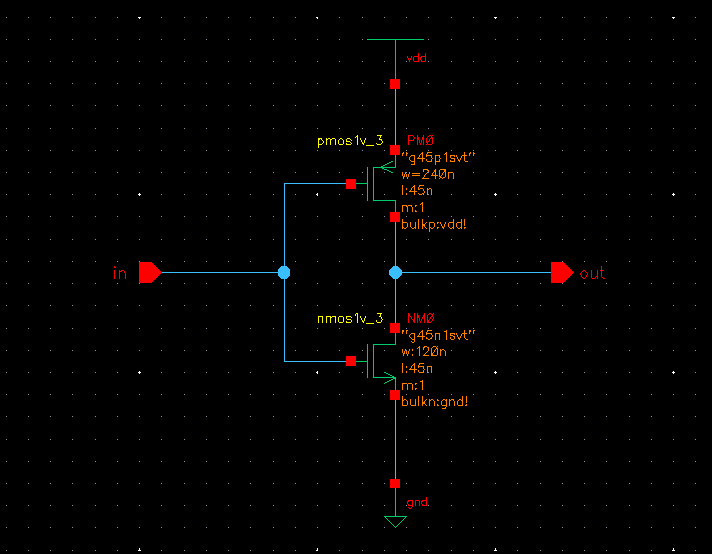
\includegraphics[width=\textwidth,height=7cm,keepaspectratio]{./figures/inverter/schematic.png}
    \caption{Schematic}\label{fig:notschematic}
\end{subfigure}
\hfill
\begin{subfigure}{0.4\textwidth}
    \centering
    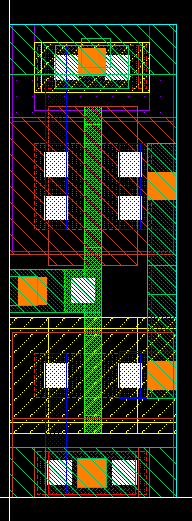
\includegraphics[width=\textwidth,height=7cm,keepaspectratio]{./figures/inverter/layout.png}
    \caption{Layout}\label{fig:notlayout}
\end{subfigure}
\caption{NOT gate circuits}
\end{figure}

\begin{figure}[H]
    \begin{subfigure}{0.48\textwidth}
        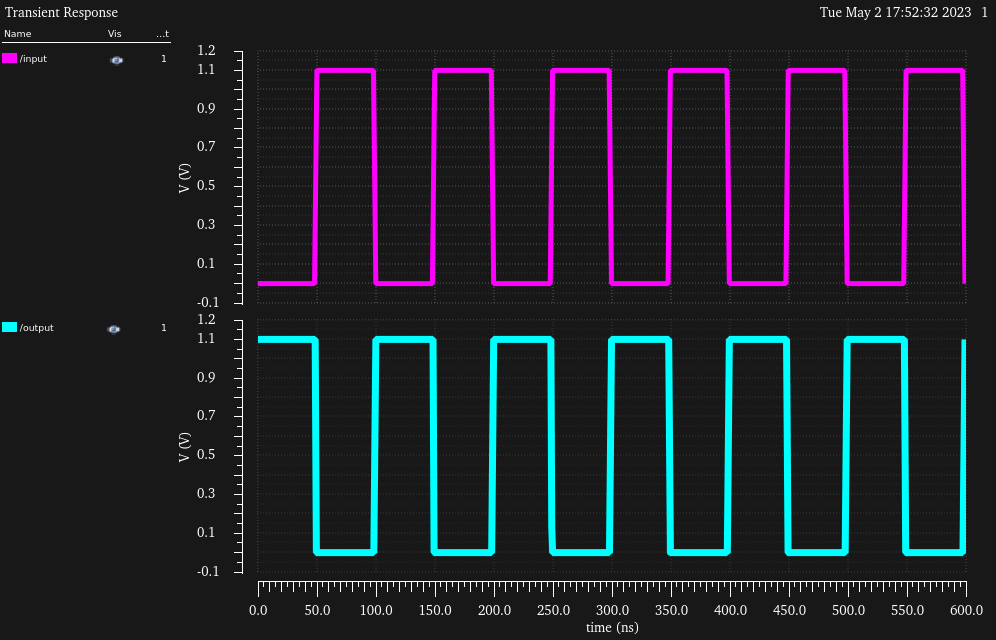
\includegraphics[width=\textwidth]{./figures/inverter/plot-schematic.png}
        \caption{Schematic}\label{fig:notplotschematic}
    \end{subfigure}
    \hfill
    \begin{subfigure}{0.48\textwidth}
        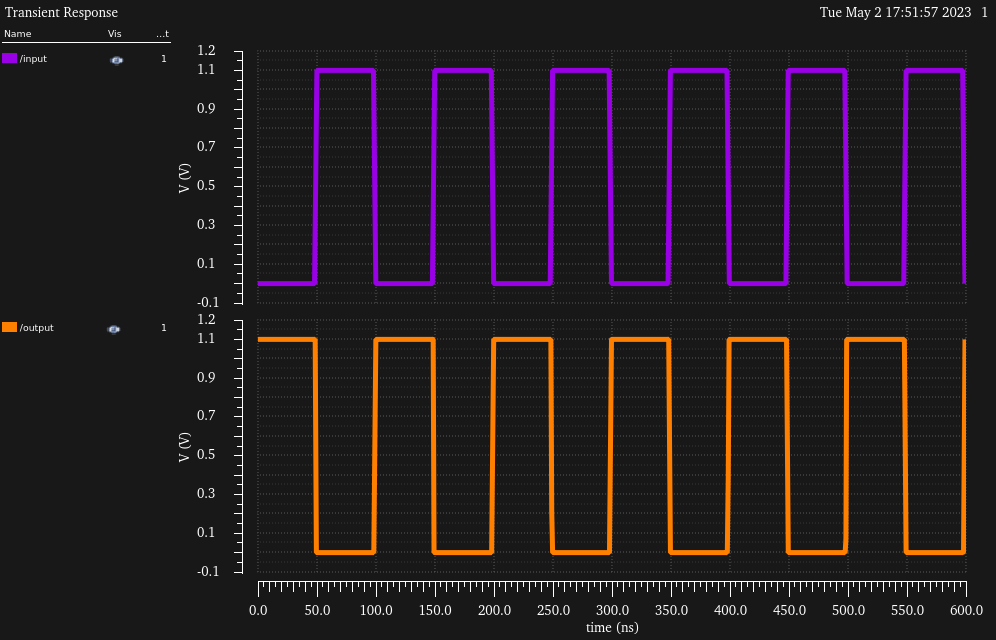
\includegraphics[width=\textwidth]{./figures/inverter/plot-layout.png}
        \caption{Layout}\label{fig:notplotlayout}
    \end{subfigure}
    \caption{NOT gate input response}
\end{figure}
\clearpage

\subsection{NAND gate}
\subsubsection{2-input}
    \begin{xltabular}{\textwidth}{YYY}
        \hline
        Peak power & Area efficiency & Transistor count \\
        \hline
        \qty{4.595}{\uW} & \qty{66.239}{\percent} & 4 \\
        \hline    
        \caption{2-input NAND gate parameters}
    \end{xltabular}

\begin{figure}[H]
    \begin{subfigure}{0.6\textwidth}
        \centering
        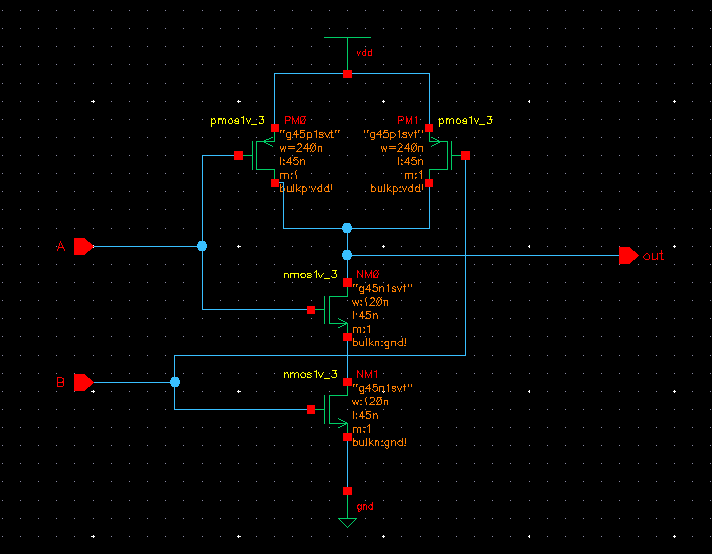
\includegraphics[width=\textwidth,height=6.5cm,keepaspectratio]{./figures/nand2/schematic.png}
        \caption{Schematic}\label{fig:nand2schematic}
    \end{subfigure}
    \hfill
    \begin{subfigure}{0.4\textwidth}
        \centering
        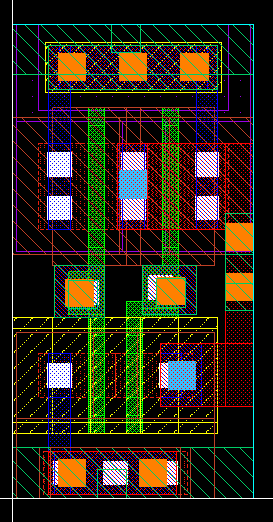
\includegraphics[width=\textwidth,height=6.5cm,keepaspectratio]{./figures/nand2/layout.png}
        \caption{Layout}\label{fig:nand2layout}
    \end{subfigure}
    \caption{2-input NAND gate circuits}
    \end{figure}
    
\begin{figure}[H]
    \centering
    \begin{subfigure}[t]{0.55\textwidth}
        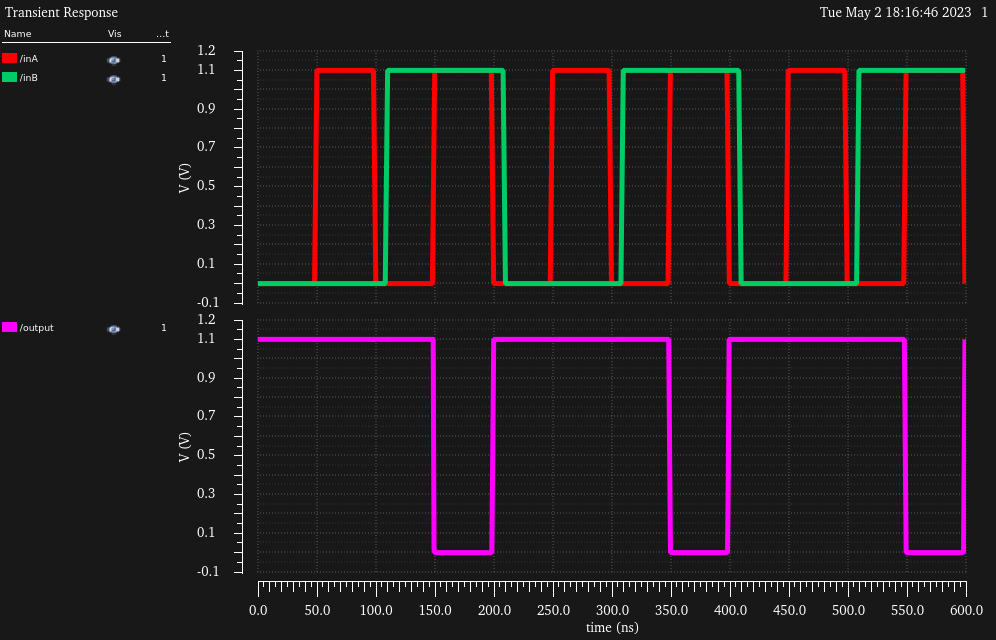
\includegraphics[width=\textwidth]{./figures/nand2/plot-schematic.png}
        \caption{Schematic}\label{fig:nand2plotschematic}
    \end{subfigure}
    \vskip\baselineskip
    \begin{subfigure}[b]{0.55\textwidth}
        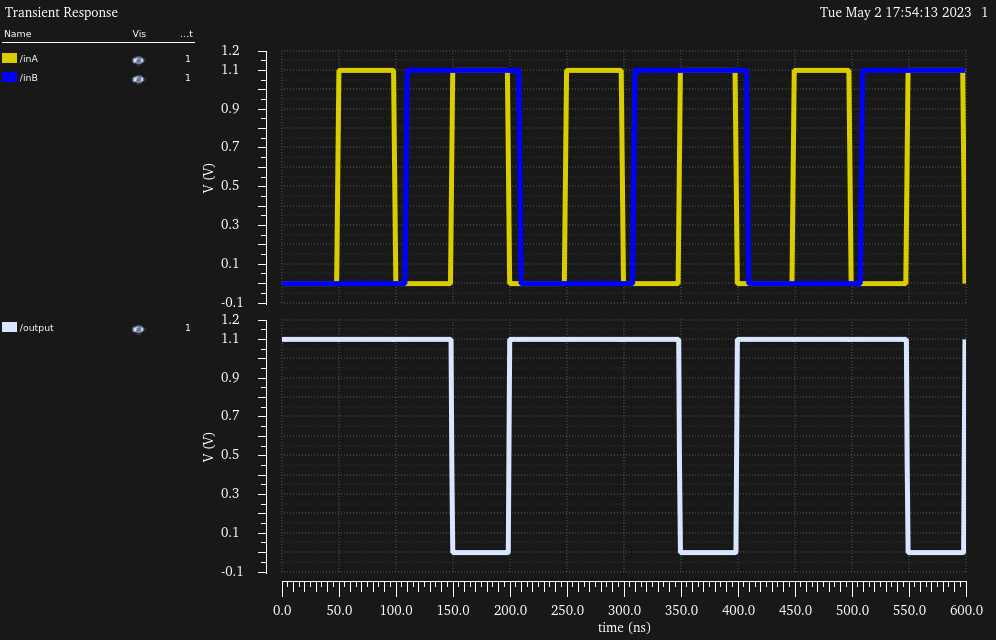
\includegraphics[width=\textwidth]{./figures/nand2/plot-layout.png}
        \caption{Layout}\label{fig:nand2plotlayout}
    \end{subfigure}
    \caption{2-input NAND gate input response}
\end{figure}

\clearpage
\subsubsection{3-input}
\begin{xltabular}{\textwidth}{YYY}
    \hline
    Peak power & Area efficiency & Transistor count \\
    \hline
    \qty{4.173}{\uW} & \qty{70.727}{\percent} & 6 \\
    \hline    
    \caption{3-input NAND gate parameters}
\end{xltabular}
\begin{figure}[H]
    \begin{subfigure}{0.6\textwidth}
        \centering
        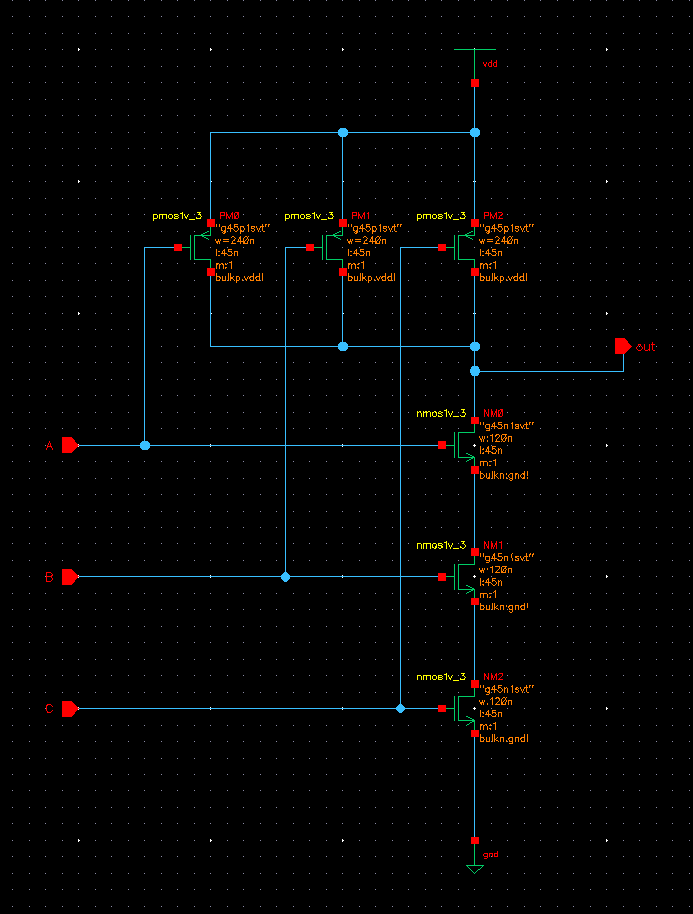
\includegraphics[width=\textwidth,height=7cm,keepaspectratio]{./figures/nand3/schematic.png}
        \caption{Schematic}\label{fig:nand3schematic}
    \end{subfigure}
    \hfill
    \begin{subfigure}{0.4\textwidth}
        \centering
        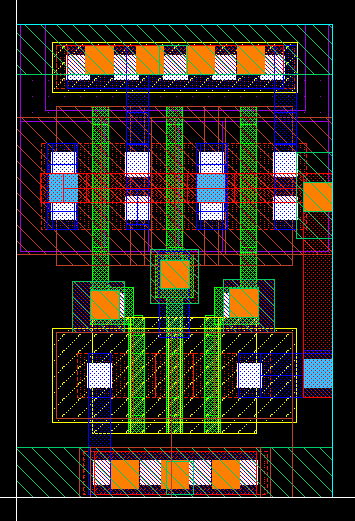
\includegraphics[width=\textwidth,height=7cm,keepaspectratio]{./figures/nand3/layout.png}
        \caption{Layout}\label{fig:nand3layout}
    \end{subfigure}
    \caption{3-input NAND gate circuits}
    \end{figure}
    
\begin{figure}[H]
    \centering
    \begin{subfigure}[t]{0.55\textwidth}
        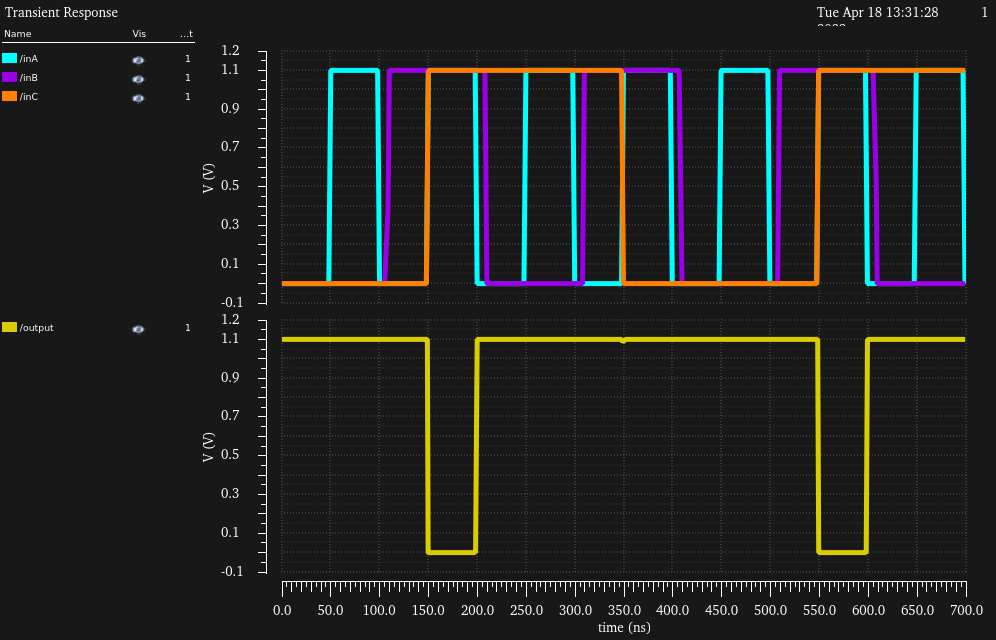
\includegraphics[width=\textwidth]{./figures/nand3/plot-schematic.png}
        \caption{Schematic}\label{fig:nand3plotschematic}
    \end{subfigure}
    \vskip\baselineskip
    \begin{subfigure}[b]{0.55\textwidth}
        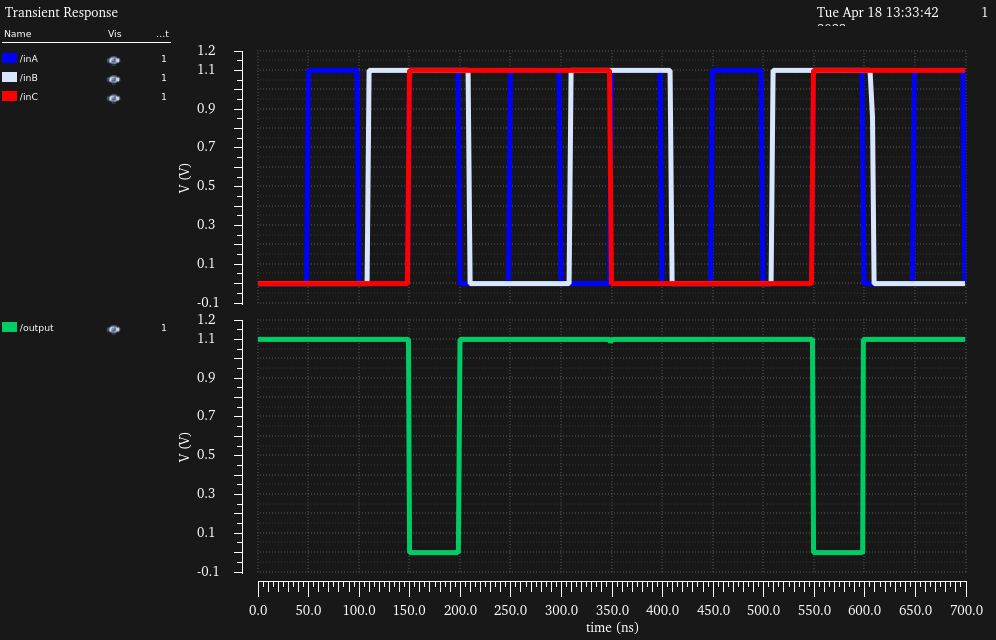
\includegraphics[width=\textwidth]{./figures/nand3/plot-layout.png}
        \caption{Layout}\label{fig:nand3plotlayout}
    \end{subfigure}
    \caption{3-input NAND gate input response}
\end{figure}

\clearpage
\subsection{NOR gate}
\subsubsection{2-input}
    \begin{xltabular}{\textwidth}{YYY}
        \hline
        Peak power & Area efficiency & Transistor count \\
        \hline
        \qty{4.329}{\uW} & \qty{64.877}{\percent} & 4 \\
        \hline    
        \caption{2-input NOR gate parameters}
    \end{xltabular}
\begin{figure}[H]
    \begin{subfigure}{0.6\textwidth}
        \centering
        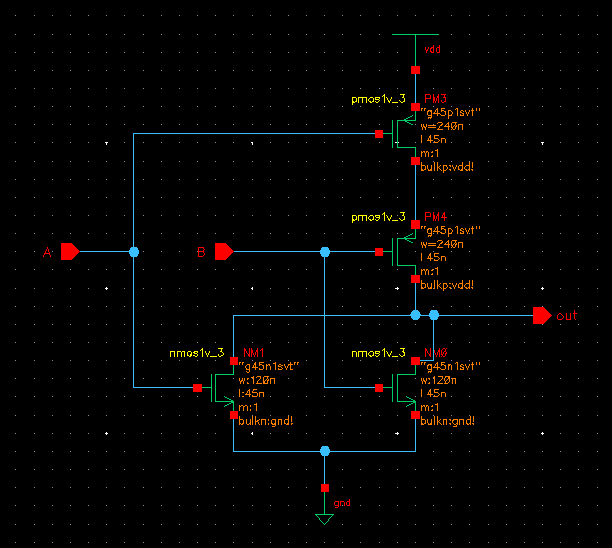
\includegraphics[width=\textwidth,height=6.5cm,keepaspectratio]{./figures/nor2/schematic.png}
        \caption{Schematic}\label{fig:nor2schematic}
    \end{subfigure}
    \hfill
    \begin{subfigure}{0.4\textwidth}
        \centering
        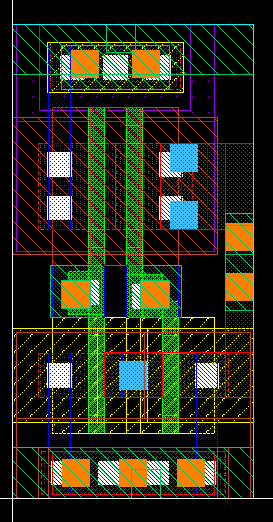
\includegraphics[width=\textwidth,height=6.5cm,keepaspectratio]{./figures/nor2/layout.png}
        \caption{Layout}\label{fig:nor2layout}
    \end{subfigure}
    \caption{2-input NOR gate circuits}
    \end{figure}
    
\begin{figure}[H]
    \centering
    \begin{subfigure}[t]{0.55\textwidth}
        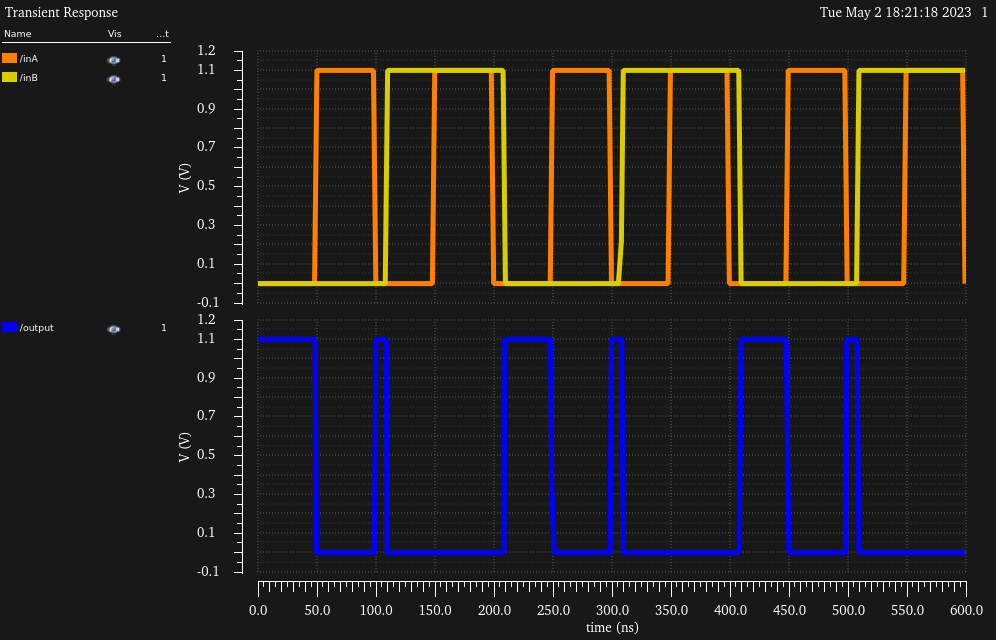
\includegraphics[width=\textwidth]{./figures/nor2/plot-schematic.png}
        \caption{Schematic}\label{fig:nor2plotschematic}
    \end{subfigure}
    \vskip\baselineskip
    \begin{subfigure}[b]{0.55\textwidth}
        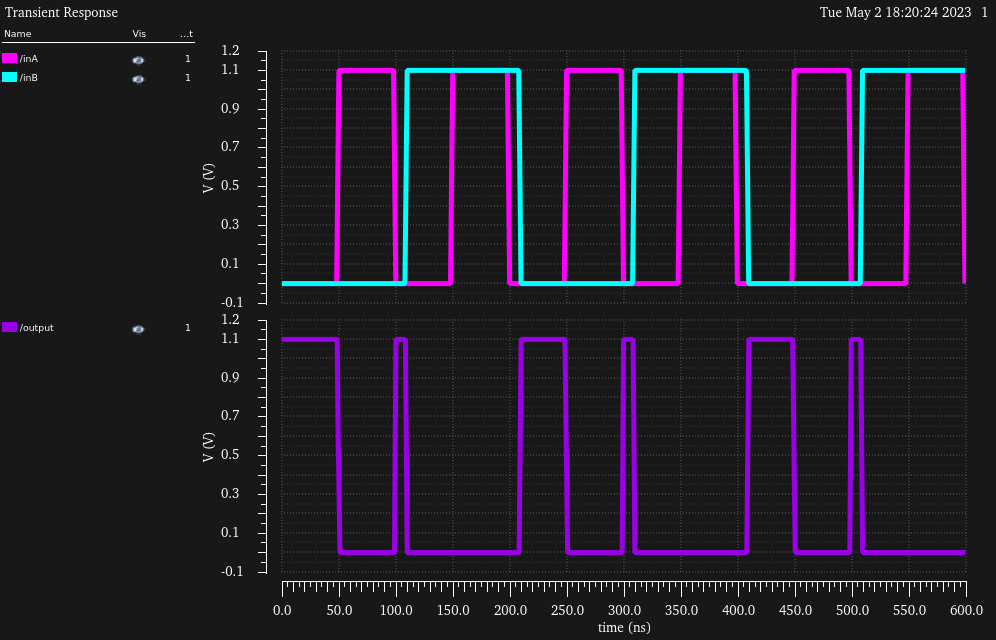
\includegraphics[width=\textwidth]{./figures/nor2/plot-layout.png}
        \caption{Layout}\label{fig:nor2plotlayout}
    \end{subfigure}
    \caption{2-input NOR gate input response}
\end{figure}

\clearpage
\subsubsection{3-input}
    \begin{xltabular}{\textwidth}{YYY}
        \hline
        Peak power & Area efficiency & Transistor count \\
        \hline
        \qty{4.911}{\uW} &  \qty{68.641}{\percent} & 6 \\
        \hline    
        \caption{3-input NOR gate parameters}
    \end{xltabular}
    
\begin{figure}[H]
    \begin{subfigure}{0.6\textwidth}
        \centering
        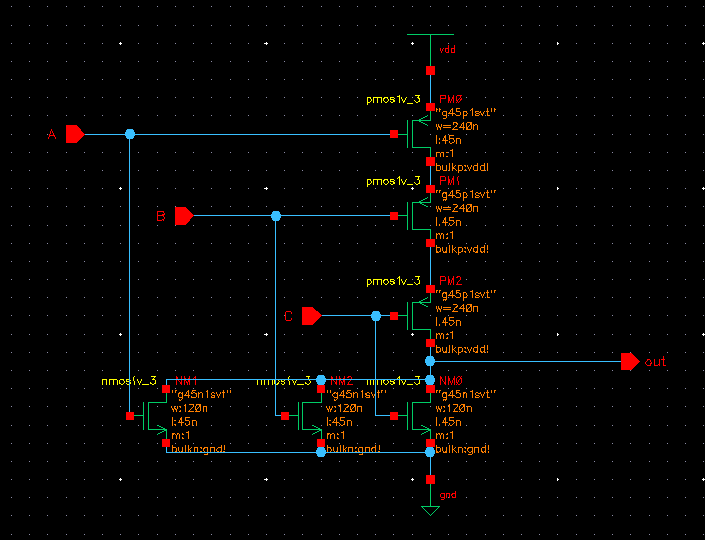
\includegraphics[width=\textwidth,height=7cm,keepaspectratio]{./figures/nor3/schematic.png}
        \caption{Schematic}\label{fig:nor3schematic}
    \end{subfigure}
    \hfill
    \begin{subfigure}{0.4\textwidth}
        \centering
        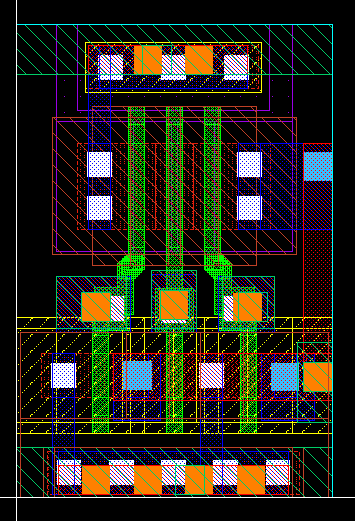
\includegraphics[width=\textwidth,height=7cm,keepaspectratio]{./figures/nor3/layout.png}
        \caption{Layout}\label{fig:nor3layout}
    \end{subfigure}
    \caption{3-input NOR gate circuits}
    \end{figure}
    
\begin{figure}[H]
    \centering
    \begin{subfigure}[t]{0.55\textwidth}
        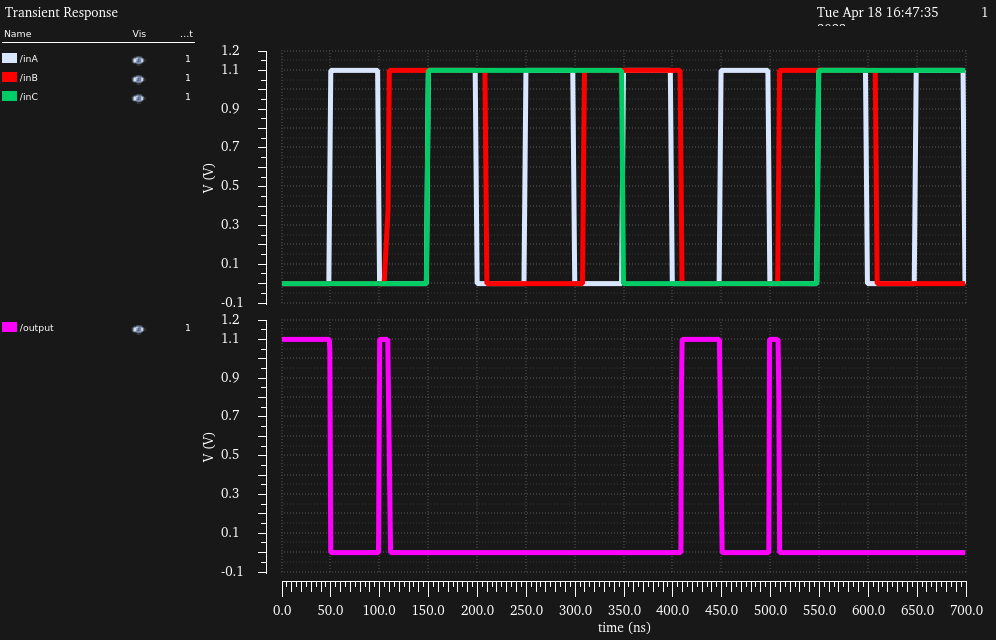
\includegraphics[width=\textwidth]{./figures/nor3/plot-schematic.png}
        \caption{Schematic}\label{fig:nor3plotschematic}
    \end{subfigure}    
    \vskip\baselineskip
    \begin{subfigure}[b]{0.55\textwidth}
        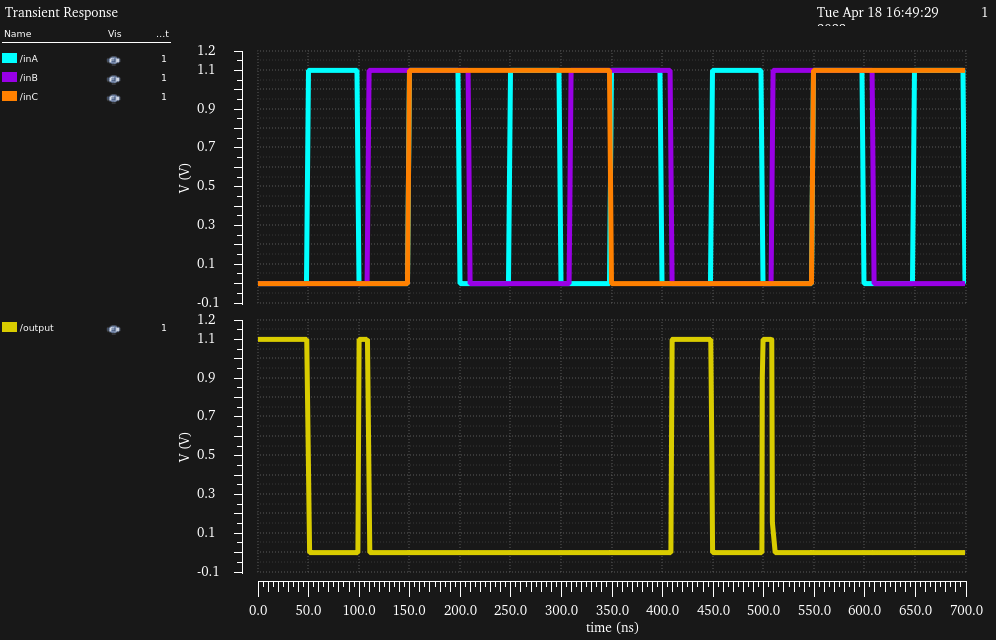
\includegraphics[width=\textwidth]{./figures/nor3/plot-layout.png}
        \caption{Layout}\label{fig:nor3plotlayout}
    \end{subfigure}
    \caption{3-input NOR gate input response}
\end{figure}



\clearpage
% \begin{landscape}
\section{Comparator design}
% \begin{xltabular}{\textwidth}{YYY}
%     \hline
%     Peak power & Area efficiency & Transistor count \\
%     \hline
%     \qty{68.189}{\uW} &  \qty{103.011}{\percent} & 6 \\
%     \hline    
%     \caption{Comparator parameters}
% \end{xltabular}
\subsection{Schematic design}
Comparator design commences with reproducing the schematic design in \cref{fig:schematic} in Virtuoso's schematic editor,
and setting up a simulation to verify the schematic functions correctly. 
\begin{figure}[H]
    \centering
    \begin{subfigure}[t]{0.39\columnwidth}
        \centering
        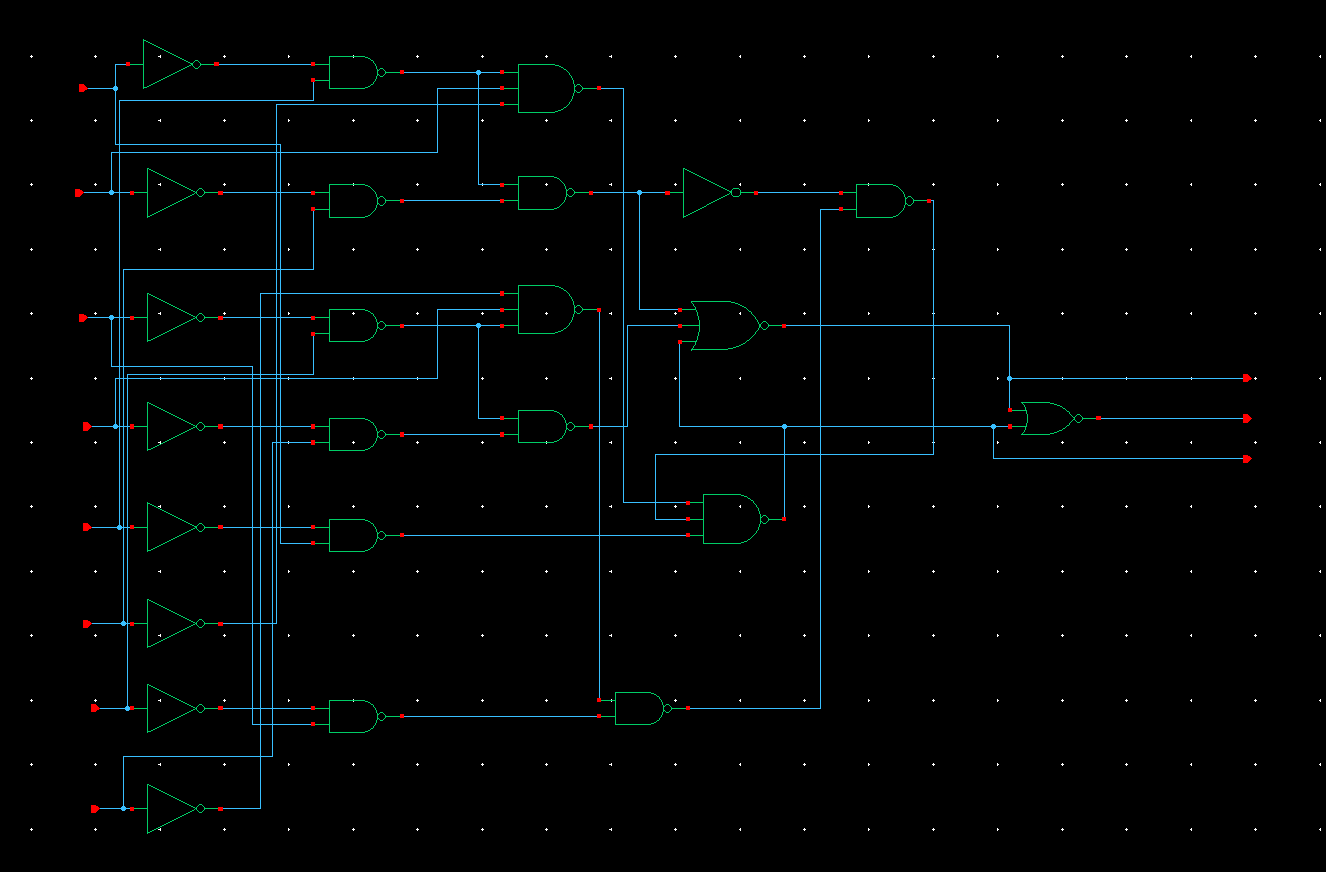
\includegraphics[width=\textwidth]{./figures/comparator/schematic.png}
        \caption{Schematic}\label{fig:comparatorschematic}
    \end{subfigure}    
    \hfill
    \begin{subfigure}[t]{0.59\columnwidth}
        \centering
        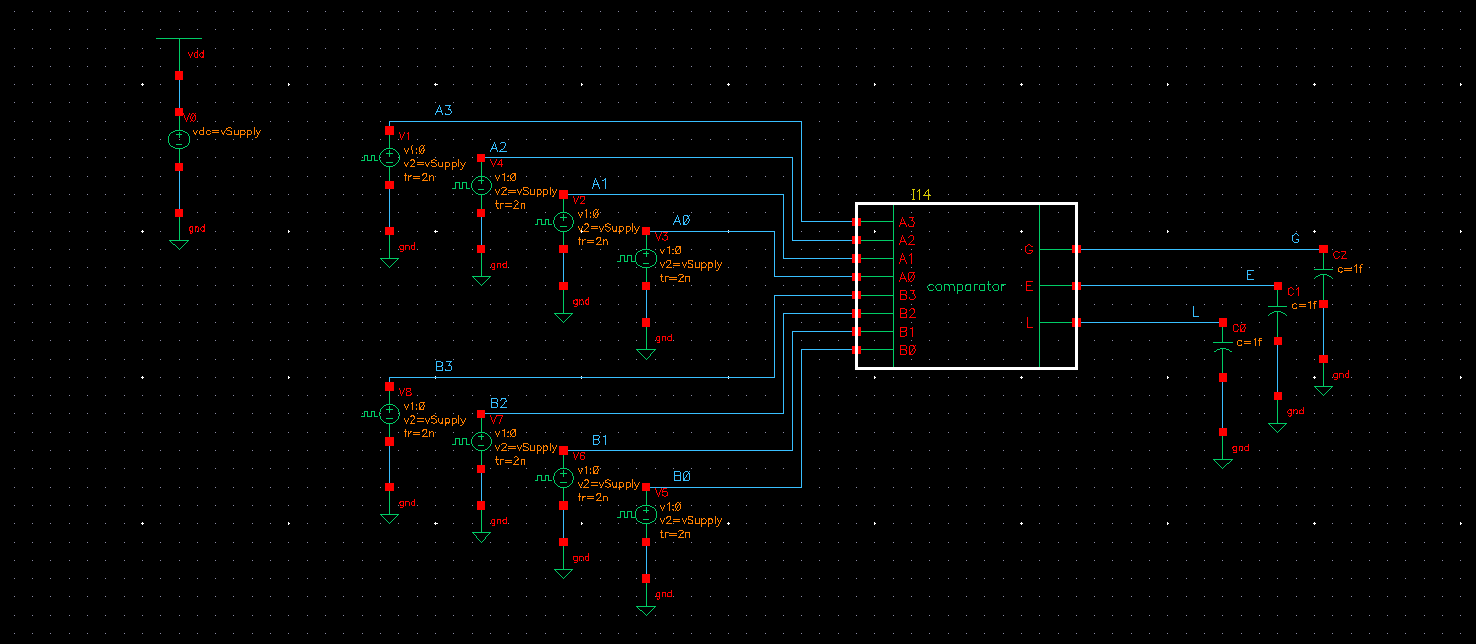
\includegraphics[width=\textwidth]{./figures/comparator/tb.png}
        \caption{Test bench}\label{fig:comparatortb}
    \end{subfigure}    
    \vskip\baselineskip
    \begin{subfigure}[b]{\columnwidth}
        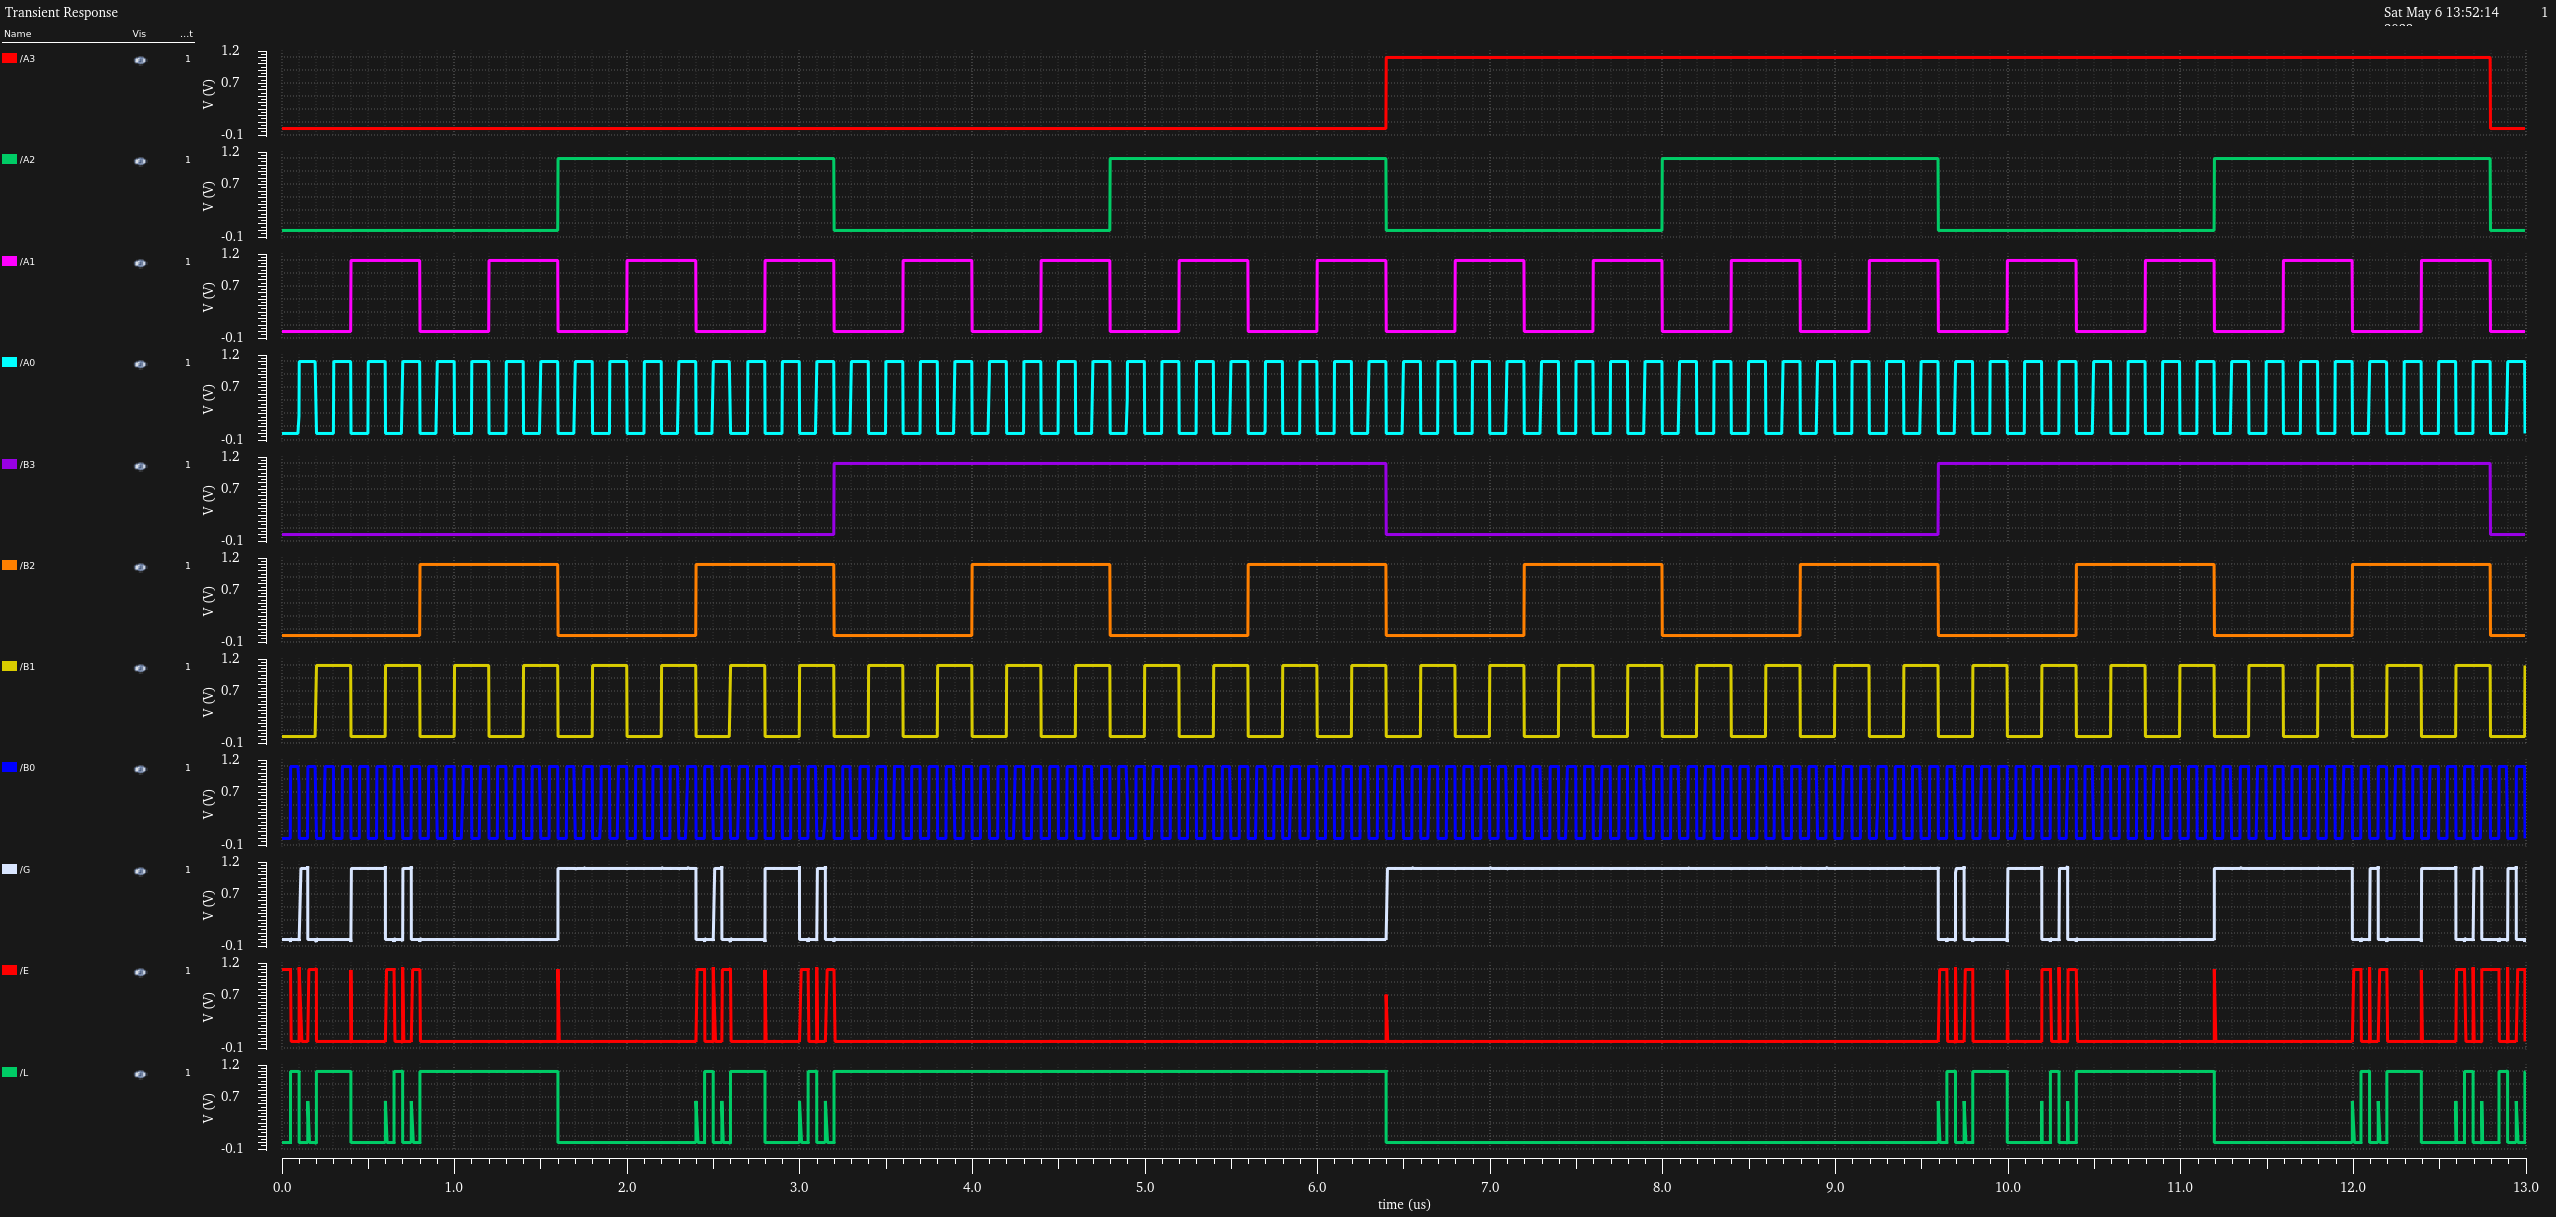
\includegraphics[width=\columnwidth]{./figures/comparator/plot-schematic.png}
        \caption{Simulation}\label{fig:comparatorplotschematic}
    \end{subfigure}
    \caption{Comparator schematic}
\end{figure}
% \end{landscape}
The simulation indicates the correct outputs for the given binary inputs. There are many instances 
in the simulation where transient undesirable outputs occur. For example, output E rises briefly, 
sometimes not even completely, when G falls and L rises at the same time. 
This is due to two reasons. In the design, a NOR gate was opted for to select the outputs rather 
than an XOR. Secondly, the rise and fall of the test bench simulation signals fall within the 
threshold voltage of the MOSFETs used. To counteract this, enough time for outputs to settle 
needs to be provided for the outputs to settle, or the comparator output can be latched 
so the output only updates on the edge of a clock. For the purposes of this design, the 
settling time will be determined after the layout is complete. 
\subsection{Layout}
The standard cell height allows for efficient routing, with vertical connections within a 
cell on the metal 3 layer, and horizontal connections between cells on metal 4 layer. 
Finally, pins and power are exposed on metal 5 layer. The pins run the height of the comparator,
so it can be connected from either end. The power rails run on metal 3, and are exposed 
at each horizontal end to metal 5. 

The cells share a well and implants, allowing them to be butted up extremely close; they can even 
be overlapped. The placement report
calculates area efficiency to be \qty{102.233}{\percent}, requiring a chip area of \qty{19.365}{\um\squared}.
\begin{landscape}
\begin{figure}[H]
    \centering
    \begin{subfigure}[t]{\columnwidth}
        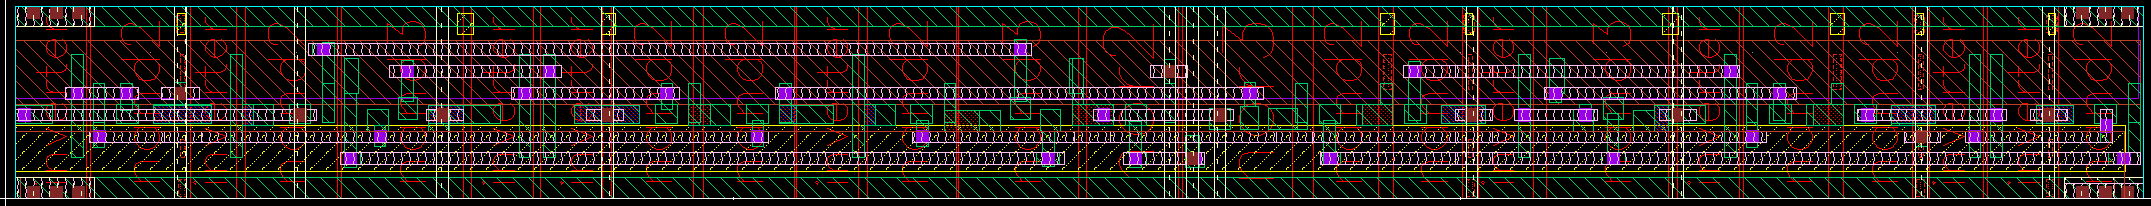
\includegraphics[width=\columnwidth]{./figures/comparator/layout.png}
        \caption{Layout}\label{fig:comparatorlayout}
    \end{subfigure}    
    \vskip\baselineskip
    \begin{subfigure}[b]{\columnwidth}
        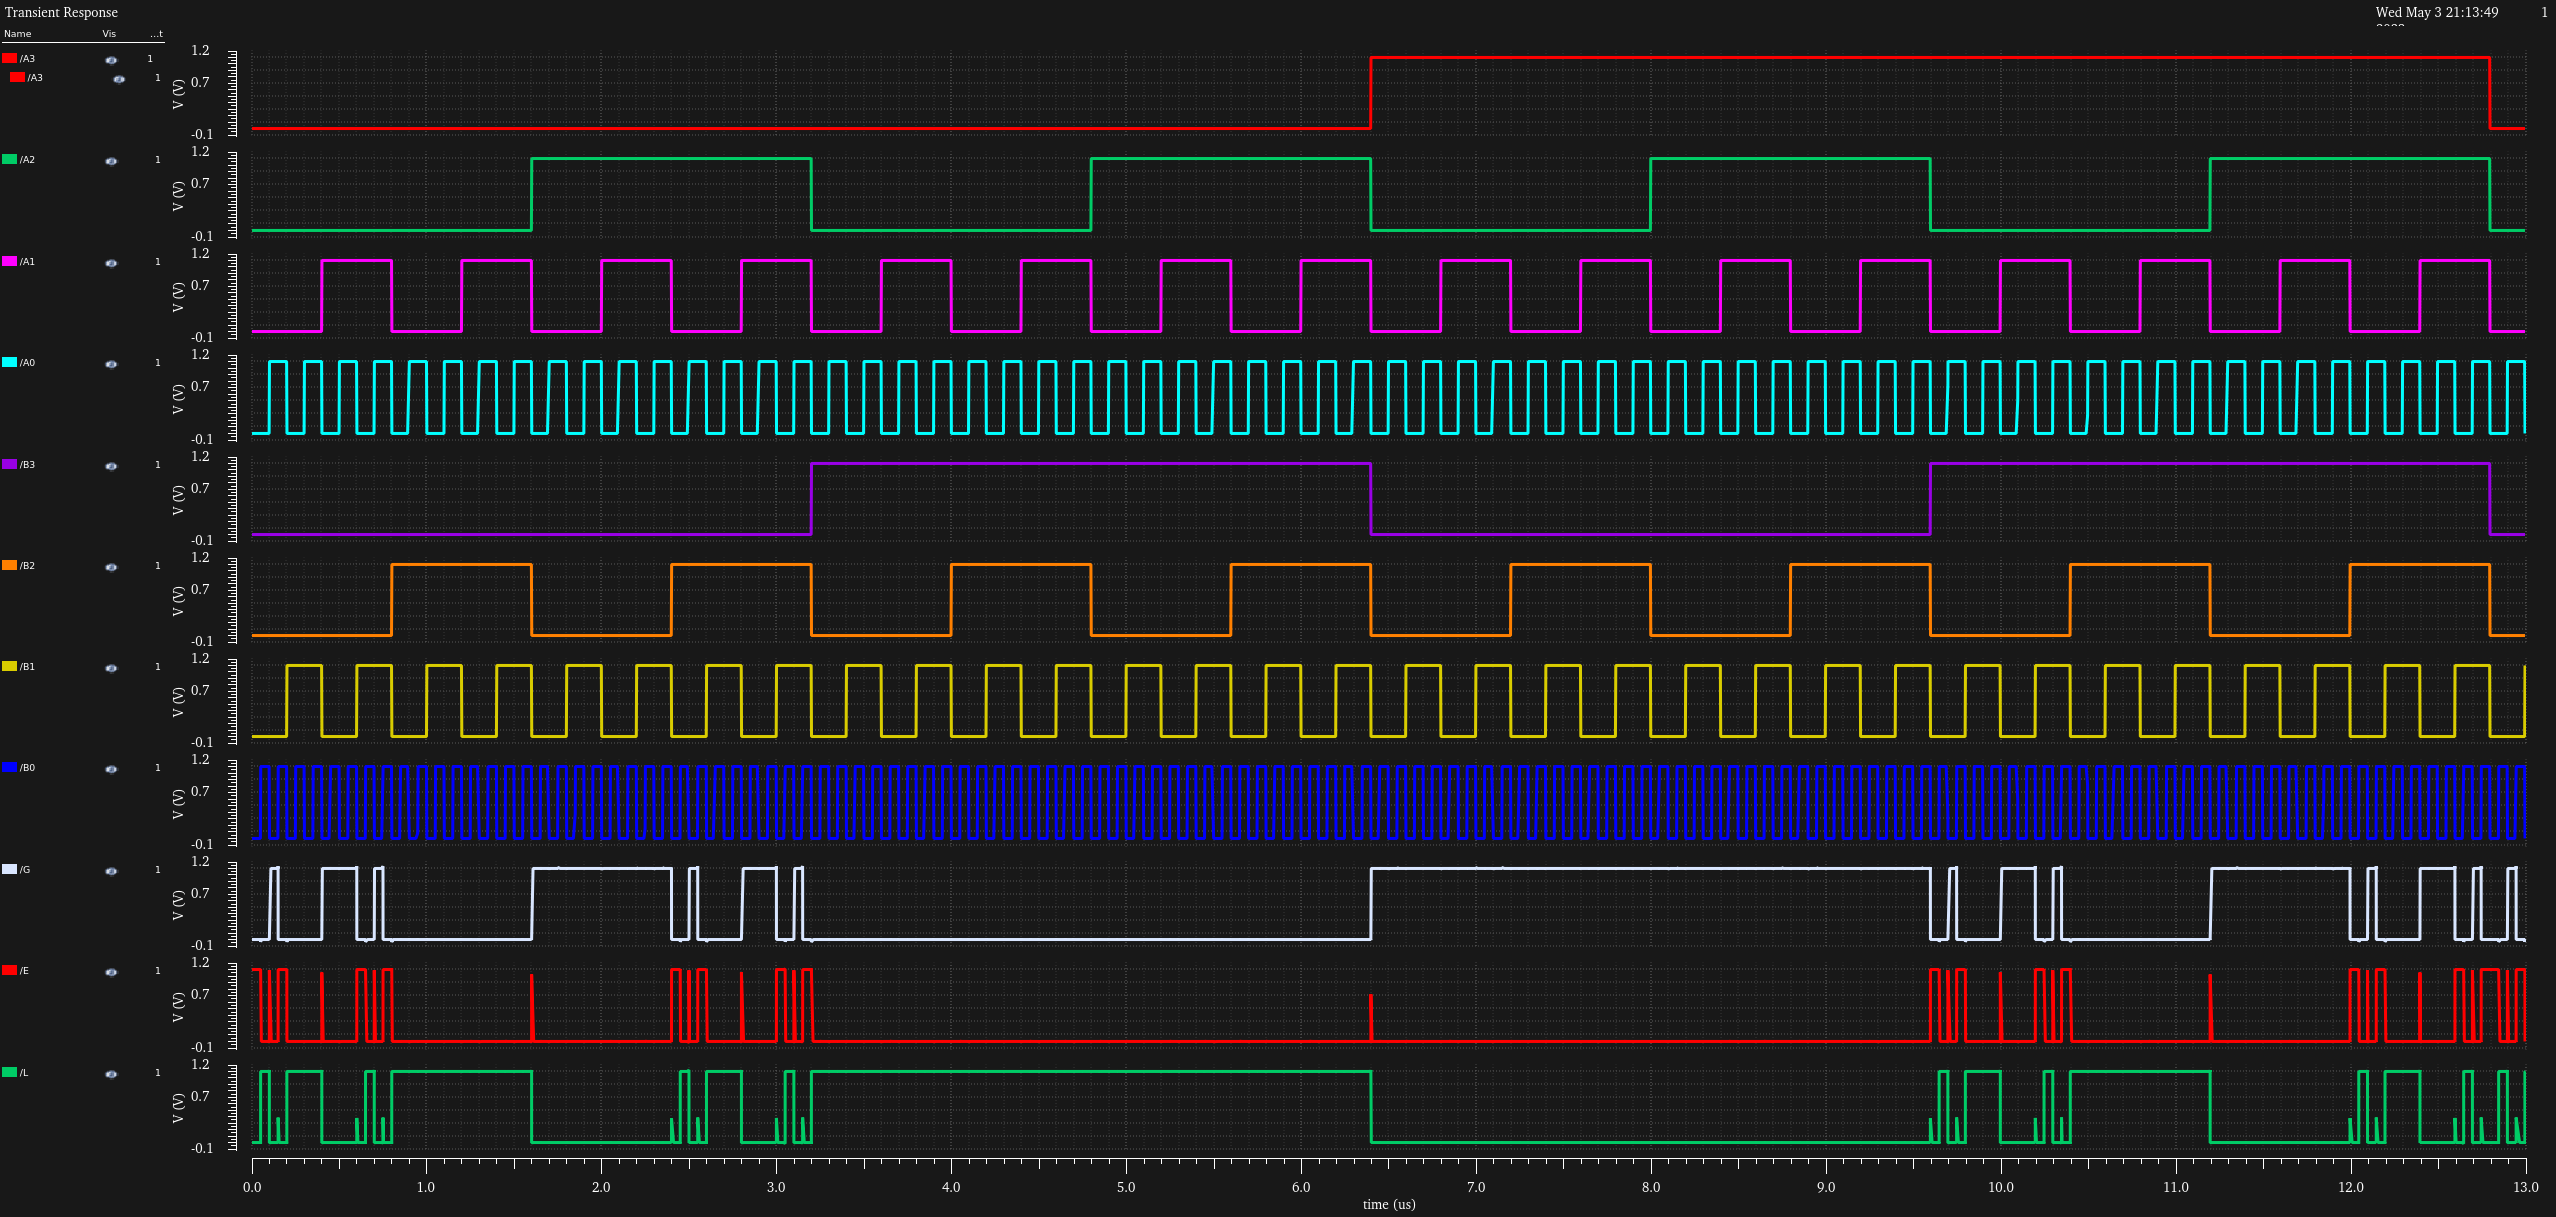
\includegraphics[width=\columnwidth]{./figures/comparator/plot-layout.png}
        \caption{Simulation}\label{fig:comparatorplotlayout}
    \end{subfigure}
    \caption{Comparator layout}
\end{figure}
\end{landscape}

\subsection{Power}
The peak dynamic power dissipation is \qty{68.189}{\uW} and occurs during switching of outputs. 
There does not appear to be a greater level of dissipation due to all outputs being high simultaneously,
suggesting that switching the NOR gate on G and E for an XNOR would have little benefit. 
\begin{figure}[H]
    \centering
    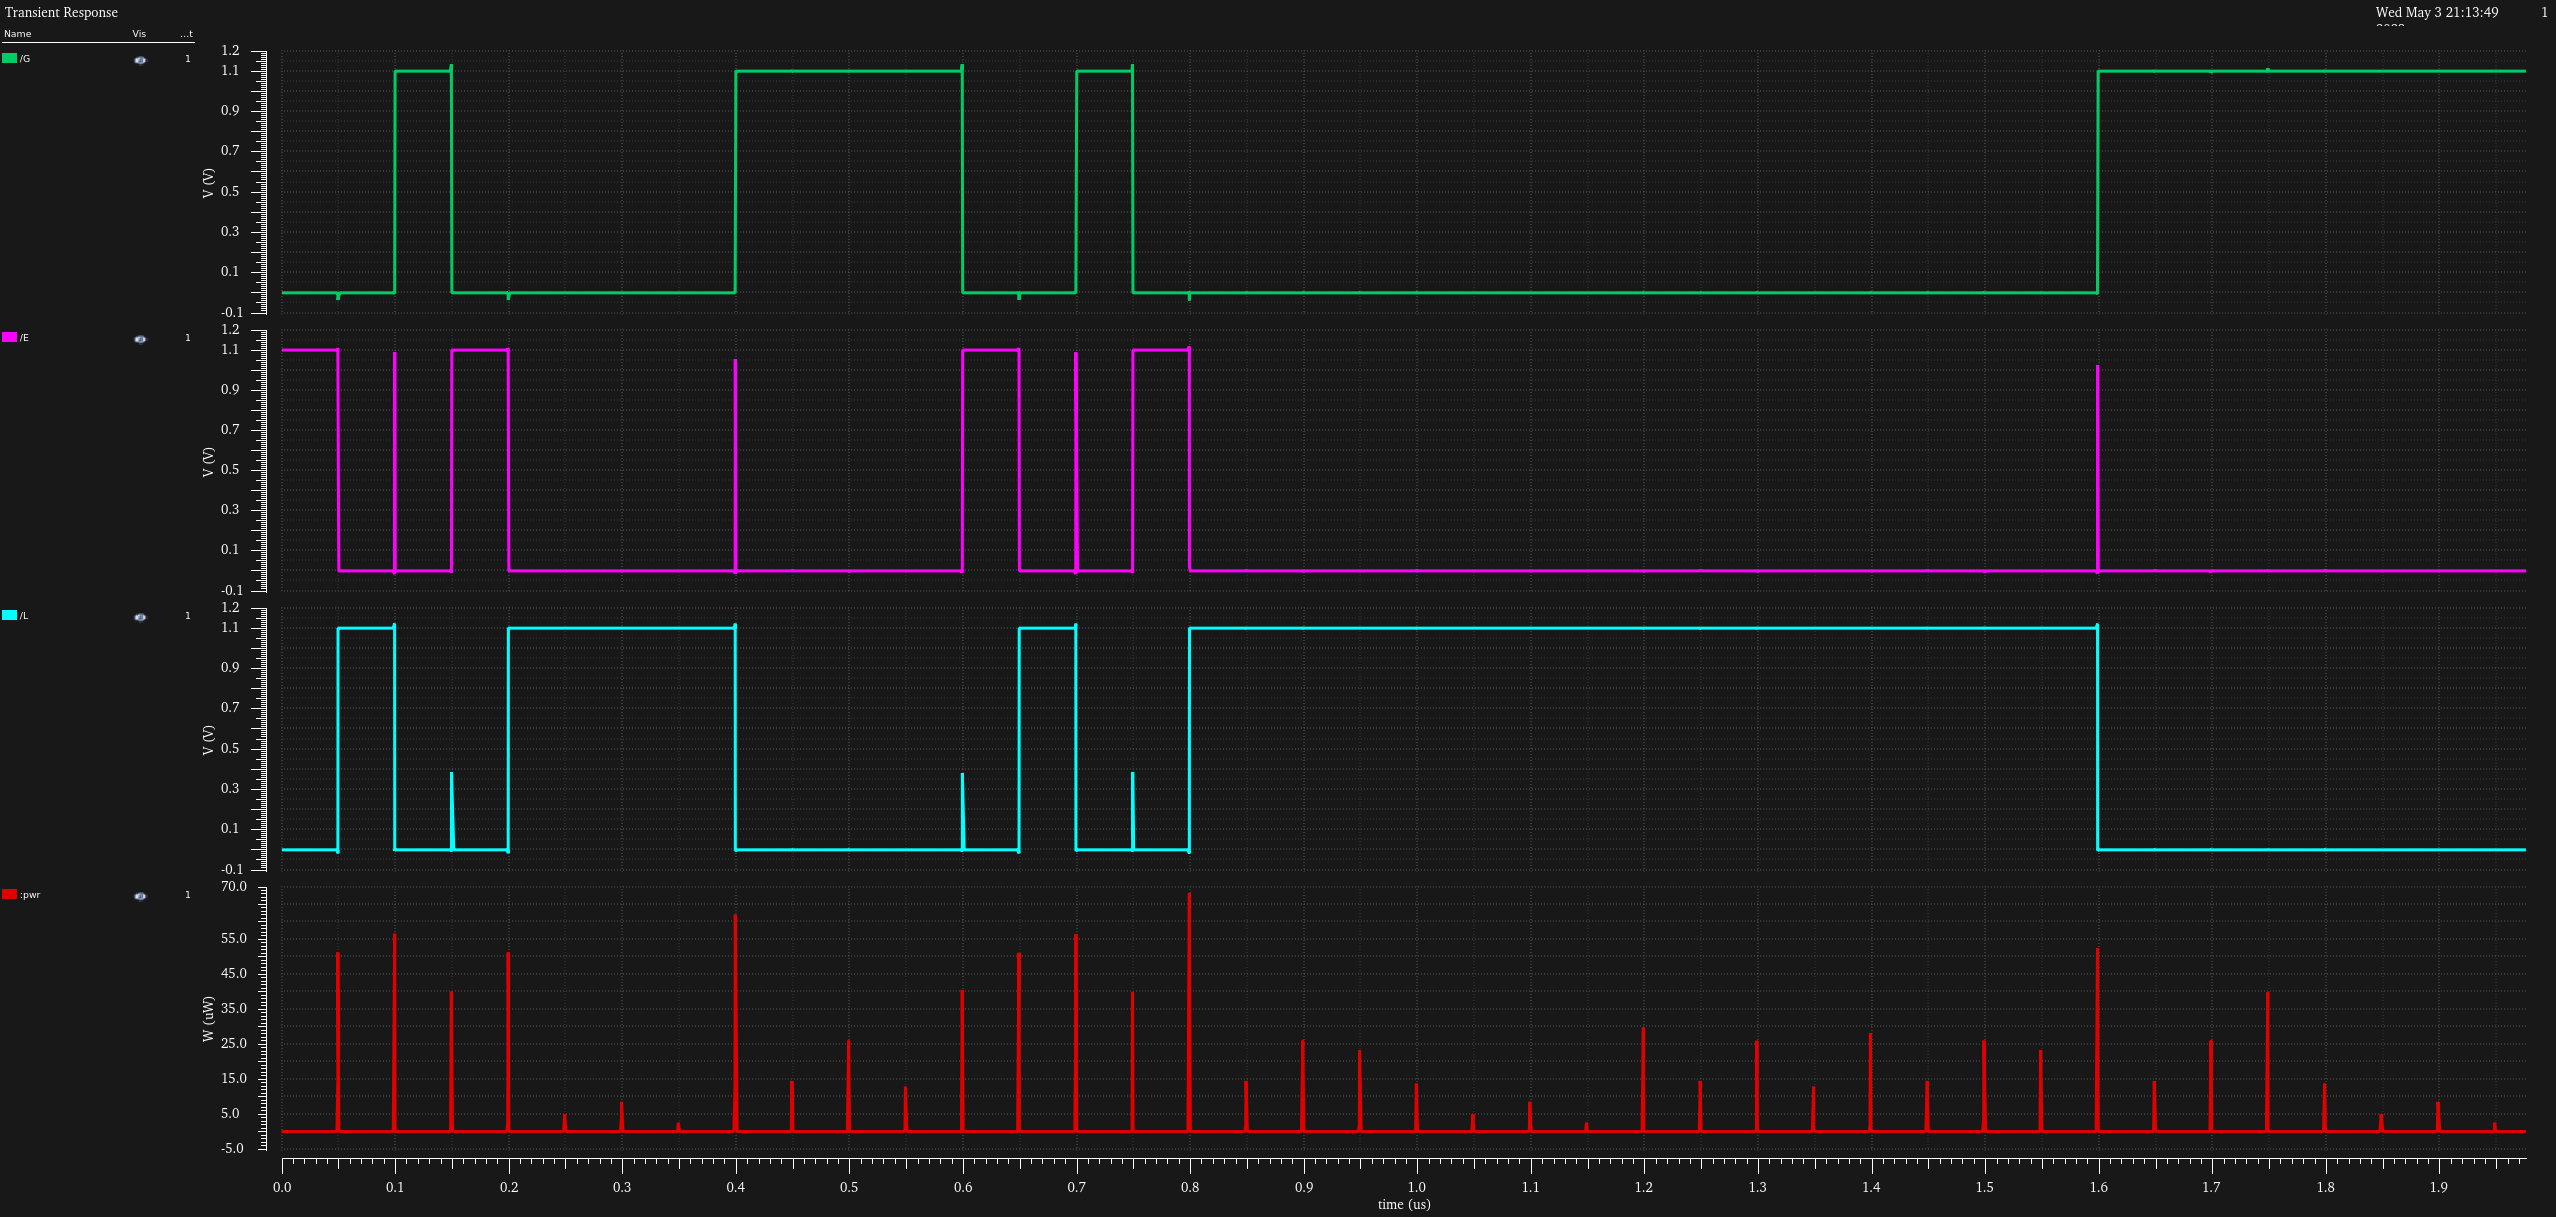
\includegraphics[width=0.95\textwidth]{./figures/comparator/pwr-outputs.png}
    \caption{Power dissipation during switching}\label{fig:comparatorpower}
\end{figure}

\subsection{Delay}
The comparator responds \qty{150}{\ps} after the input reaches \qty{50}{\percent} of vSupply (\qty{0.55}{\V}), and 
settles after an additional \qty{200}{\ps}. Considering settling time for transient outputs, readings 
are available from the comparator after, at earliest \qty{350}{\ps}, or comfortably after \qty{400}{\ps}. 
This suggests a maximum possible clock speed of \qty{2.857}{\GHz}.
\begin{figure}[H]
    \centering
    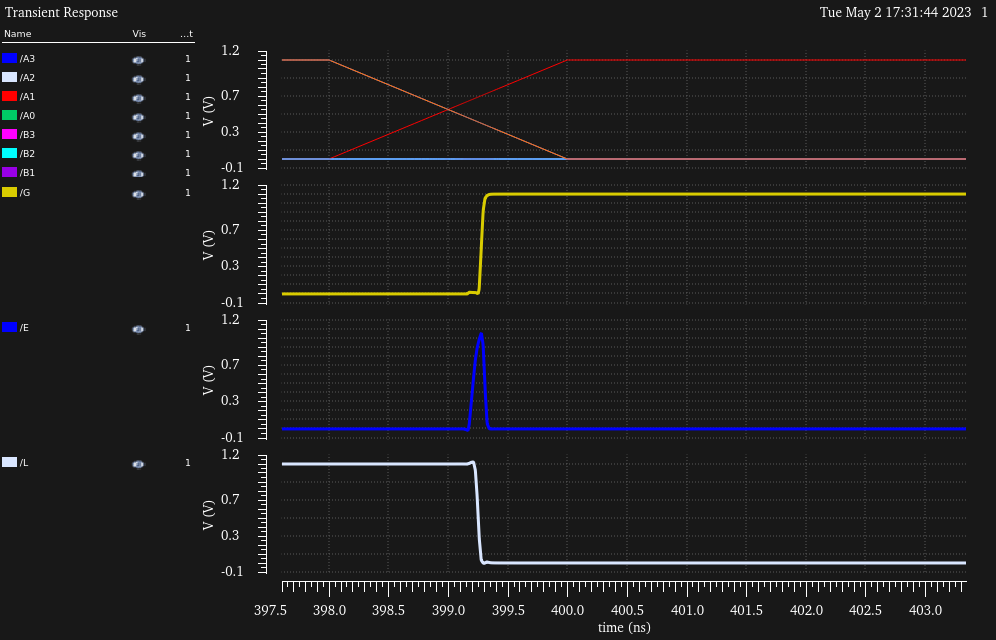
\includegraphics[width=0.95\textwidth]{./figures/comparator/sim-response-layout.png}
    \caption{Transient output}\label{fig:comparatortransient}
\end{figure}


\clearpage
\section{Evaluation}

\begin{xltabular}{\textwidth}{YYYYYY}
    \hline
    Peak power & Area efficiency & Chip area & Transistor count & Delay & Recommended clock \\
    \hline
    \qty{68.189}{\uW} & \qty{102.233}{\percent} & \qty{19.365}{\um\squared} & 86 & \qty{400}{\ps} & $\leqslant$\qty{2.5}{\GHz}  \\
    \hline    
    \caption{Performance metrics}
\end{xltabular} 

The comparator as a whole appears to function quite well. 
It responds appropriately and quickly to the input of two 4-bit numbers, A and B, to set 
the outputs G (greater), E (equal), or L (lesser). 
Die area is low and utilisation is high, achieved by overlapping standard cells.
The design uses a reasonably low number of transistors, at 86, spread across five 
gate ICs. While designs using fewer transistors are possible, they may introduce 
complexity when maintaining standardised cells or perform slower. 

\subsection{Standard cells}
The design leverages the use of standard cells to attain the extremely high area
efficiency. The cells share a common n-well, implants, and power rails, allowing 
gates to be overlapped. While each individual gate's area efficiency can be improved, 
the aim for standardisation allows the top cell to recoup those losses. The large diffusions 
required may also increase the expense of manufacture. 
The use of taller cells may allow for this expense to be reduced, however that would 
have to balanced against the total area used. 

A downside of designing in this manner is that it leads to routing with little to no 
flexibility to accommodate changes. Using the comparator as a standard cell itself 
may require adjustment of sizing, which may prove difficult. 

\subsection{Routing}
The pins and rails for each cell are exposed on metal 3. Routing on the top cell
then uses metal 4 to move horizontally between cells. As the rails are on 
the same metal layer as the vertical routing, the maximum number of horizontal lines that 
can be supported is reduced. The comparator falls within the level of complexity that 
can be supported, however it is close to the limit of what is possible with a single line
layout given the maximum number of horizontal tracks (six) is reached. 

Routing can be improved by exposing the rails on a different layer to the internal pins (thereby 
allowing overlapping), and increasing the standard cell height for more complex designs. For particularly 
complex designs, routing may not be possible across the cells, in which case pins may need to move 
to be commonly accessible from a routing channel.

\subsection{Power dissipation}
Compact routing across the cells additionally lead to a low value of power dissipation during 
switching. Due to the level of complexity of the design, and thereby the total number of transistors used,
the static power dissipation is in the region of yW and negligible when analysing the comparator by itself.  

\subsection{Delay}
The minimum delay required was calculated to be \qty{100}{\ps}, which is 3.5 times smaller 
than the observed minimum delay, \qty{350}{\ps}. This indicates that there may be areas for 
improvement in the design to minimise this, although managing this without sacrificing on 
other aspects like area utilisation may be difficult to balance. 
One such improvement may be to change the NOR gate across G and E for an XNOR, potentially allowing 
a quicker response by limiting transient outputs. 



 % eval

\nocite{*}

\printbibliography

\end{document}